% Drawing 74/05-13 -- folder 74, batch 05, archive page 88 (PDF page 89).
% Transcription: Un bitriangle sur les sommets $(ba')$, $(bb')$, $(aa')$, $(ab')$ : côtés horizontaux $(ba')\text{---}(bb')$ et $(aa')\text{---}(ab')$, une diagonale $(bb')\text{---}(aa')$ en trait fin, deux amorces de l'autre diagonale.
% Kind: bitriangle with one thin diagonal. Method 2 (schematic redraw from the facsimile). Status: ok.
% Notes: Horizontal sides (ba')-(bb') and (aa')-(ab'), the diagonal (bb')-(aa') in a thin stroke, and two starts of the other diagonal.
% Coordinates: 1 unit = 1 mm = 1/100 of the crop width (bbox in page fractions: [0.38, 0.18, 0.62, 0.27]).
% Redrawn by Claude (claude-opus-5-5), issue #73, 2026-11-07; not checked by a human; not compiled (no TeX in the session).
% Rights: reproduces part of the work -- behind RENDER_TRANSCRIPTS, never published by itself.
\documentclass[tikz,border=3pt]{standalone}
\usepackage{amsmath,amssymb}
\usetikzlibrary{patterns,arrows.meta}
\tikzset{pencil/.style={black!45}, struck/.style={black!35}, mark/.style={circle,draw,inner sep=1.3pt}, pt/.style={circle,fill,inner sep=0.9pt}, opt/.style={circle,draw,fill=white,inner sep=1.1pt}}
\begin{document}
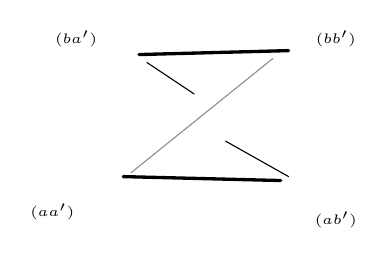
\begin{tikzpicture}[x=1mm,y=1mm,line cap=round,line join=round,font=\scriptsize]
\node[inner sep=1pt] at (33,-20) {\tiny $(ba')$};
\node[inner sep=1pt] at (66,-20) {\tiny $(bb')$};
\node[inner sep=1pt] at (30,-42) {\tiny $(aa')$};
\node[inner sep=1pt] at (66,-43) {\tiny $(ab')$};
\draw[very thick] (41,-22) -- (60,-21.5);
\draw[very thick] (39,-37.5) -- (59,-38);
\draw[pencil] (58,-22.5) -- (40,-37);
\draw (42,-23) -- (48,-27);
\draw (52,-33) -- (60,-37.5);
\end{tikzpicture}
\end{document}
